
\chapter{Cryptography Overview}
\label{chapter:cryptographyoverview}

% Provide a brief overview
\section{Overview}
Before delving into the details of various applications for secure physical system design,
it is necessary to define and understand several different
cryptographic primitives, as they form a foundation on which the applications build. The following sections present a brief
introduction to the necessary cryptographic primitives that will be used in the rest of the thesis.

% Encryption operations
\section{Encryption}
It is often necessary to scramble and protect data so that only certain parties, such as those who
possess a key value, can de-scramble and read the protected data. This might be necessary when
sending any sort of sensitive data, such as financial records or e-mail messages. Presumably, if a 
person does not have the correct key value, he or she will not be able to scramble or unscramble
the data properly.

The act of scrambling the data is called \emph{encryption}. The corresponding act of descrambling
encrypted data is called \emph{decryption}.

Encryption and decryption operations and relevant parameters are denoted using the following notation below.

\begin{align}
C = E_{K_E}(M) \\
M = D_{K_D}(C)
\end{align}

Above, C is the \emph{ciphertext}, or encrypted text.  
M is the message or \emph{plaintext}. 
E represents the \emph{encryption algorithm}, of which there are several types. This algorithm takes plaintext as a parameter and returns ciphertext.
D represents the \emph{decryption algorithm}, which takes ciphertext and return plaintext.
K represents the \emph{key value}. $K_E$ is used with the encryption algorithm, while $K_D$ is used with the decryption algorithm.

A sender would use his plaintext message to generate the ciphertext and transmit it. The receiver would then process the received data using the decryption
algorithm and then be able to successfully recover the plaintext message.

% Symmetric key encryption
\subsection{Symmetric Encryption}
Symmetric encryption is a fairly intuitive method of using encryption. In this style of encryption,
both the sender and receiver share the same key value, K. In this scenario $K_E = K_D$. There are several,
different symmetric encryption algorithms, such as AES~\cite{AES}, DES~\cite{DES}, Blowfish~\cite{Blowfish}, and many others.
For my purposes, I typically use AES. It is fast and considered fairly secure.

One difficulty with symmetric encryption is the establishment of a shared symmetric keys between the two communicating parties.
If there is a secure channel between the sender and recipient, it is trivial to simply send the value $K$ across the secure channel.
If there is no secure channel however, there are protocols, such as the Diffie-Hellman Key Exchange~\cite{diffiehellmankeyexchange} algorithm.
This is a somewhat cumbersome step to do for every communication. Additionally, a party must maintain a different symmetric key for each
other party he or she wishes to contact.

% Asymmetric key encryption
\subsection{Asymmetric Encryption}
Asymmetric encryption is an interesting cryptographic building block. In this system, $K_E \neq K_D$. Typically,
$K_E$ is a \emph{public key}, while $K_D$ is a \emph{private key}. That is, $K_E$ may be published somewhere publicly,
which then allows anyone to encrypt messages. However, without $K_D$, these messages cannot be decrypted. As such, (typically) only one person
will have $K_D$. 

This is a useful system because it allows anyone to send a given person an encrypted message easily: Simply retrieve the public key,
encrypt the message, and send it to the recipient. Unlike symmetric encryption, there is no need for a protocol to establishing a shared symmetric
key. This greatly alleviates the problems that key management systems impose.

There are several systems for asymmetric encryption schemes. One popular scheme is RSA ~\cite{RSA}. In this scheme, a user picks a value which becomes
$K_D$ and uses that to derive $K_E$. It is considered unreasonably difficult to derive $K_D$ from $K_E$ though, which makes this scheme secure.
Interested users may refer to \cite{RSA} for more specific details on the RSA scheme.
% Block ciphers
%\subsection{Block Ciphers}

% Stream ciphers
%\subsection{Stream Ciphers}

% Digital Signatures
\section{Digital Signatures}
An important ability when sending messages is for one party to "sign" the message. This
allows a recipient to be confident that the sender is actually who he claims to be, much
like a physical signature on a physical document. Due to the fact that electronic media
is so easily manipulated, it is somewhat difficult to ensure that the sender of electronic
materials is who he claims to be.

Several algorithms exist that can be used for digital signatures. In general terms, the signer
will know some secret, or a private key,
 which he will use to sign messages. He will
also publish some value related to the private key, known as the public key. When he wishes
to send a signed message, the sender will use his private key to perform some operation
on the message and send the message and result of the operation to the recipient. 
The recipient will then perform some operation on what he 
received from the sender, using the sender's public key. If the signature is authentic, the
recipient will be able to determine this, or if not, this will also become more apparent.
Figure~\ref{fig:signing} illustrates this process.

\begin{figure}[!ht]
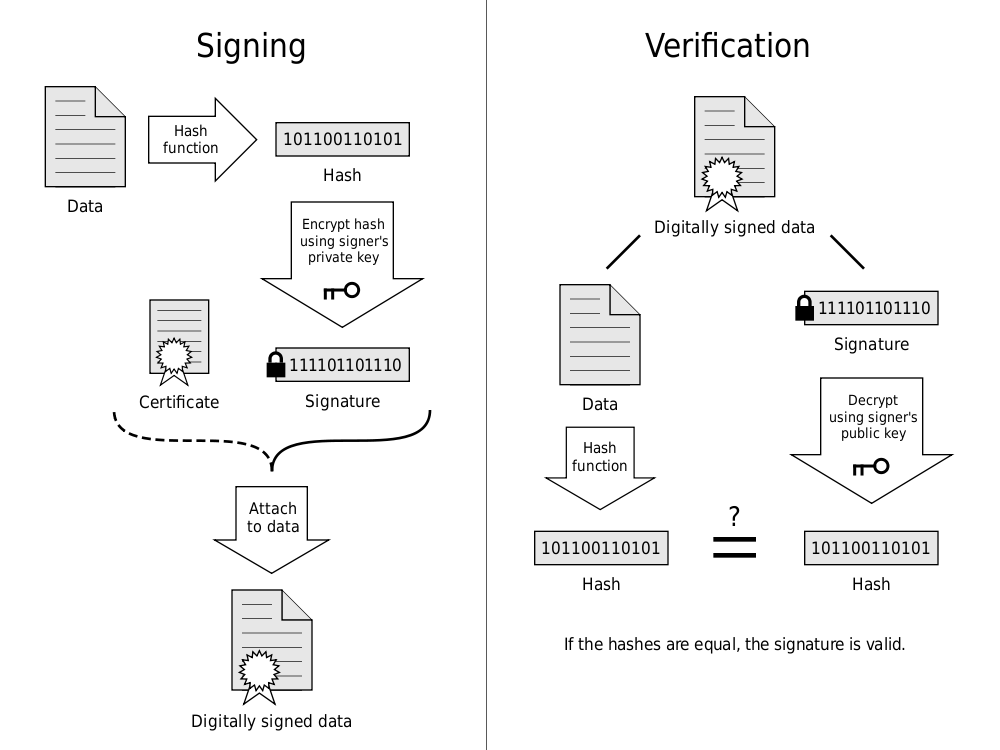
\includegraphics[width=400px]{images/signing.png}
\caption{A graphical representation of the digital signature process \cite{signing}}
\label{fig:signing}
\end{figure}


% ZKPK
\section{Zero Knowledge Proof of Knowledge}
A party might need to prove that it knows some value. Sometimes it is acceptable
to simply reveal the value, but in other cases, this might not be acceptable. For instance, imagine
if Peggy, Victor, and Eve are in the same room. Victor wants to make sure Peggy knows his phone number,
but does not want Eve to learn her phone number. Peggy cannot simply repeat Victor's phone
number, lest Eve overhear and write it down. In this case, Peggy will use what is called a
\textit{zero knowledge proof of knowledge} or ZKPK.

A ZKPK is a way to prove for one party to prove to another that it knows a secret without actually
revealing the secret. A basic use case was just described, but there are many reasons why a ZKPK
might be useful. A ZKPK can be used when there is concern that a man-in-the-middle is present
and could determine the secret (as was the case in the previous example), but to defeat this,
encryption is usually a better alternative. Where a ZKPK is very useful is when the sender does not
want to reveal the secret to the recipient. So in a similar example, say that Peggy wanted to prove to
Victor that she knew her own phone number, but did not want to give it to Victor. This is when the
use of a ZKPK is most applicable.

There are multiple different schemes that implement ZKPK behaviors. 
The scheme the author is most familiar with is called the Feige-Fiat-Shamir Identification Scheme (FFS). 
The scheme works using modular arithmetic, similar to the RSA algorithm above.
Interested readers are referred to the original paper in \cite{ffs} for more details. 

% Committments
\section{Commitment Schemes}
It is often necessary for a party to be bound to some decision it has made in the past, but without
actually revealing that decision. For example, suppose Alice and Bob are talking on the phone and
want to flip a coin to solve a dispute. This is clearly subject to much distrust, since whoever flips the
coin could lie about the result so he or she always wins.
This is where a commitment scheme would be useful.

More formally, a commitment scheme is defined as a two step procedure. In the first step, a value
is chosen and \textit{committed}. This \textit{commitment} does not reveal the value chosen, so it
may be publicly published somewhere if desired. The second step is \textit{revealing}. In this step,
the private value is revealed and then verified against the commitment previously made.

In the coin-flipping example, a commitment scheme could be employed as follows. Alice would 
secretly decide whether to call heads or tails. She would then \textit{commit} this value to Bob. Recall
that this commitment does not reveal Alice's choice. Bob would then tell Alice the result of the coin
flip. Alice would then tell Bob what she committed previously. Bob checks this value against Alice's
commitment. If the value checks out, Bob accepts that Alice actually did call that value.

Commitment schemes are often used in conjunction with zero knowledge proof of knowledge schemes; 
A prover proves to a verifier that he knows the value used to generate a commitment without having to reveal
to the verifier such value. The verifier only accepts the committed value.
The method the author is most familiar with
is known as Pedersen commitments. Readers interested in more details of this scheme are referred
to the original paper \cite{pedersen}.

